\documentclass[8pt]{article}

\usepackage[a4paper]{geometry}
\usepackage{fullpage}
\usepackage{graphicx}
\usepackage{float}


\title{DMML Coursework C}
\author{Joseph Davidson \\ 071729468 \\ MEng Software Engineering}
\date{}

\begin{document}

  \maketitle

  \section{Introduction}
    This is the report for DMML 2010 coursework c set by Professor De Wilde. This coursework concerned itself with
    the construction of a decision tree that is used to select Facebook adverts for users based on certain attributes.
    To this end, a training set of 14 records was selected, each of which having one of 3 adverts. 4 attributes that
    seemed the most relevant to the adverts were also chosen.

    The 3 adverts selected were:
    \begin{itemize}
      \setlength{\itemsep}{1pt}
      \setlength{\parskip}{0pt}
      \setlength{\parsep}{0pt}
      \item A dating website.
      \item A car insurance website.
      \item An advert for coupons that offer deals to Edinburgh students.
    \end{itemize}

    The 4 attributes selected:
    \begin{itemize}
      \setlength{\itemsep}{1pt}
      \setlength{\parskip}{0pt}
      \setlength{\parsep}{0pt}
      \item Relationship Status.
      \item Current Location.
      \item Education.
      \item Age\footnote{While Age itself is not an attribute, the age can be inferred by the birthday attribute that is
      part of a Facebook page.}.
    \end{itemize}

        
   \begin{center}
    \begin{table}[ht!]
       \centering
        \caption{The 14 records selected}
        \begin{tabular}{|c|c|c|c|c||c|}
          \hline
          \textbf{Record} & \textbf{RS} & \textbf{CL} &\textbf{Education} & \textbf{Age} & \textbf{Selected Advert} \\
           \hline  
           1 & Single        &Edinburgh  &University & 20 & Edinburgh Student Deals \\
           2 & Relationship  &London     &University & 19 & Car Insurance           \\
           3 & Single        &Glasgow    &University & 21 & Dating Website          \\
           4 & Single        &Edinburgh  &University & 20 & Edinburgh Student Deals \\
           5 & Relationship  &Glasgow    &School     & 18 & Car Insurance           \\
           6 & Single        &Edinburgh  &School     & 18 & Dating Website          \\
           7 & Single        &Edinburgh  &University & 19 & Dating Website          \\
           8 & Relationship  &London     &None       & 21 & Car Insurance           \\
           9 & Relationship  &Glasgow    &University & 19 & Car Insurance           \\
           10& Single        &London     &None       & 21 & Dating Website          \\
           11& Single        &Edinburgh  &None       & 19 & Dating Website          \\
           12& Relationship  &Edinburgh  &School     & 18 & Edinburgh Student Deals \\
           13& Single        &Glasgow    &School     & 18 & Car Insurance           \\
           14& Relationship  &London     &University & 20 & Car Insurance           \\
           \hline
         \end{tabular}

    \end{table}
   \end{center}

  \section{Calculating the root}
    All of the calculations for building the tree were entropy and gain calculations. These formulae were
    taken from the lecture notes and are reiterated below.

    \begin{equation}
      Entropy(S)\equiv \sum_{i=1}^{c} -p_{i}log_{2}p_{i}
    \end{equation}
    \begin{equation}
      Gain(S,A)\equiv Entropy(S) - \sum_{v\in Values(A)} \frac{|S_v|}{|S|}Entropy(S_v)
    \end{equation}

    First the attribute of the root had to be calculated. This was done by working out the entropy over the
    entire set ($Entropy([3_{ES},6_{CI},5_{DS}]) = 1.53$ where ES = Edinburgh Student Deals, CI = Car Insurance and
    DS = Dating Site) and then calculating the gain from sorting on a particular attribute.

    \subsection{Gain on Relationship Status}

      \begin{description}
        \setlength{\itemsep}{1pt}
        \setlength{\parskip}{0pt}
        \setlength{\parsep}{0pt}
        \item[$Entropy(S_{Single})$] $\equiv Entropy([2_{ES},1_{CI},5_{DS}]) = 1.298$
        \item[$Entropy(S_{Relationship})$] $\equiv Entropy([1_{ES},5_{CI},0_{DS}]) = 0.65$
        \item[$Gain(S,RS)$] $= 0.509$ 
      \end{description} 

    \subsection{Gain on Current Location}

      \begin{description}
        \setlength{\itemsep}{1pt}
        \setlength{\parskip}{0pt}
        \setlength{\parsep}{0pt}
        \item[$Entropy(S_{Edinburgh})$] $\equiv Entropy([3_{ES},0_{CI},3_{DS}]) = 1$
        \item[$Entropy(S_{Glasgow})$] $\equiv Entropy([0_{ES},3_{CI},1_{DS}]) = 0.811$
        \item[$Entropy(S_{London})$] $\equiv Entropy([0_{ES},3_{CI},1_{DS}]) = 0.811$
        \item[$Gain(S,CL)$] $= 0.638$
      \end{description}


    \subsection{Gain on Education}

      \begin{description}
        \setlength{\itemsep}{1pt}
        \setlength{\parskip}{0pt}
        \setlength{\parsep}{0pt}
        \item[$Entropy(S_{University})$] $\equiv Entropy([2_{ES},3_{CI},2_{DS}]) = 1.556$
        \item[$Entropy(S_{School})$] $\equiv Entropy([1_{ES},2_{CI},1_{DS}]) = 1.5$
        \item[$Entropy(S_{None})$] $\equiv Entropy([0_{ES},1_{CI},2_{DS}]) = 0.918$
        \item[$Gain(S,Edu)$] $= 0.1267$
      \end{description}

    \subsection{Gain on Age}

      \begin{description}
        \setlength{\itemsep}{1pt}
        \setlength{\parskip}{0pt}
        \setlength{\parsep}{0pt}
        \item[$Entropy(S_{18})$] $\equiv Entropy([1_{ES},2_{CI},1_{DS}]) = 1.5$
        \item[$Entropy(S_{19})$] $\equiv Entropy([0_{ES},2_{CI},2_{DS}]) = 1$
        \item[$Entropy(S_{20})$] $\equiv Entropy([2_{ES},1_{CI},0_{DS}]) = 0.918$
        \item[$Entropy(S_{21})$] $\equiv Entropy([0_{ES},1_{CI},2_{DS}]) = 0.918$
        \item[$Gain(S,Age)$] $= 0.4222$
      \end{description}

    The best gain experienced by sorting on attributes was from using Current Location. This is why it was selected
    as the root attribute.


  \section{The Second Level}
    For the second level of the tree, I had to do entropy and gain calculations for each of the remaining attributes
    paired with each leaf of the root node. Which happened to be $3^2 = 9$. Each leaf now had a reduced set of $S$, which
    is shown below:

    \begin{description}
      \item [$S_{Edinburgh}$] $ = [D1,D4,D6,D7,D11,D12]$ 
      \item [$S_{Glasgow}$] $ = [D3,D5,D9,D13]$
      \item [$S_{London}$] $ = [D2,D8,D10,D14]$
    \end{description}

    The specific calculations for determining the next node for each branch is below, but here are the results.
    The bolded results are the ones that were selected as the next node in each branch.

    \begin{description}
      \setlength{\itemsep}{1pt}
      \setlength{\parskip}{0pt}
      \setlength{\parsep}{0pt}
      \item [] $Gain(S_{Edinburgh},RS) = 0.196$
      \item [] $Gain(S_{Edinburgh},Edu) = 0.2$
      \item [] $\mathbf{Gain(S_{Edinburgh},Age) = 0.666}$
    \end{description}

    \begin{description}
      \setlength{\itemsep}{1pt}
      \setlength{\parskip}{0pt}
      \setlength{\parsep}{0pt}
      \item [] $Gain(S_{Glasgow},RS) = 0.311$
      \item [] $Gain(S_{Glasgow},Edu) = 0.311$
      \item [] $\mathbf{Gain(S_{Glasgow},Age) = 0.811}$
    \end{description}

    \begin{description}
      \setlength{\itemsep}{1pt}
      \setlength{\parskip}{0pt}
      \setlength{\parsep}{0pt}
      \item [] $\mathbf{Gain(S_{London},RS)= 0.811}$
      \item [] $Gain(S_{London},Edu) = 0.311$
      \item [] $Gain(S_{London},Age) = 0.311$
    \end{description}


    \subsection{Relationship Status Calculations}

      \subsubsection{Edinburgh}
         $Entropy(S_{Edinburgh}) \equiv Entropy([3,0,3])=1$

        \begin{description}
          \setlength{\itemsep}{1pt}
          \setlength{\parskip}{0pt}
          \setlength{\parsep}{0pt}
          \item[$Entropy(S_{Edinburgh/Single})$] $\equiv Entropy([2_{ES},0_{CI},3_{DS}]) = 0.970$
          \item[$Entropy(S_{Edinburgh/Relationship})$] $\equiv Entropy([1_{ES},0_{CI},0_{DS}]) = 0$
          \item[$Gain(S_{Edinburgh},RS)$] $= 0.196$
        \end{description}

      \subsubsection{Glasgow}
        $Entropy(S_{Glasgow}) \equiv Entropy([0,3,1])=0.811$ 

        \begin{description}
          \setlength{\itemsep}{1pt}
          \setlength{\parskip}{0pt}
          \setlength{\parsep}{0pt}
          \item[$Entropy(S_{Glasgow/Single})$] $\equiv Entropy([0_{ES},1_{CI},1_{DS}]) = 1$
          \item[$Entropy(S_{Glasgow/Relationship})$] $\equiv Entropy([0_{ES},2_{CI},0_{DS}]) = 0$
          \item[$Gain(S_{Glasgow},RS)$] $= 0.311$
        \end{description}


      \subsubsection{London}
         $Entropy(S_{London}) \equiv Entropy([0,3,1])=0.811$

        \begin{description}
          \setlength{\itemsep}{1pt}
          \setlength{\parskip}{0pt}
          \setlength{\parsep}{0pt}
          \item[$Entropy(S_{London/Single})$] $\equiv Entropy([0_{ES},0_{CI},1_{DS}]) = 0$
          \item[$Entropy(S_{London/Relationship})$] $\equiv Entropy([0_{ES},3_{CI},0_{DS}]) = 0$
          \item[$Gain(S_{London},RS)$] $= 0.811$
        \end{description} 


    \subsection{Education Calculations}

      \subsubsection{Edinburgh}
         $Entropy(S_{Edinburgh}) \equiv Entropy([3,0,3])=1$

        \begin{description}
          \setlength{\itemsep}{1pt}
          \setlength{\parskip}{0pt}
          \setlength{\parsep}{0pt}
          \item[]$Entropy(S_{Edinburgh/University})\equiv Entropy([2_{ES},0_{CI},1_{DS}]) = 0.918$
          \item[]$Entropy(S_{Edinburgh/School})\equiv Entropy([1_{ES},0_{CI},1_{DS}]) = 1$
          \item[]$Entropy(S_{Edinburgh/None})\equiv Entropy([0_{ES},0_{CI},1_{DS}]) = 0$
          \item[]$Gain(S_{Edinburgh},Edu)= 0.2$
        \end{description}


      \subsubsection{Glasgow}
        $Entropy(S_{Glasgow}) \equiv Entropy([0,3,1])=0.811$
   
        \begin{description}
          \setlength{\itemsep}{1pt}
          \setlength{\parskip}{0pt}
          \setlength{\parsep}{0pt}
          \item[]$Entropy(S_{Glasgow/University})\equiv Entropy([0_{ES},1_{CI},1_{DS}]) = 1$
          \item[]$Entropy(S_{Glasgow/School})\equiv Entropy([0_{ES},2_{CI},0_{DS}]) = 0$
          \item[]$Entropy(S_{Glasgow/None})\equiv Entropy([0_{ES},0_{CI},0_{DS}])$ - This evaluated as 0.
          \item[]$Gain(S_{Glasgow},Edu)= 0.311$
        \end{description}

      \subsubsection{London}

        $Entropy(S_{London}) \equiv Entropy([0,3,1])=0.811$

        \begin{description}
          \setlength{\itemsep}{1pt}
          \setlength{\parskip}{0pt}
          \setlength{\parsep}{0pt}
          \item[]$Entropy(S_{London/University})\equiv Entropy([0_{ES},2_{CI},0_{DS}]) = 0$
          \item[]$Entropy(S_{London/School})\equiv Entropy([0_{ES},0_{CI},0_{DS}]) = 0$ - This evaluated as 0.
          \item[]$Entropy(S_{London/None})\equiv Entropy([0_{ES},1_{CI},1_{DS}]) = 1$
          \item[]$Gain(S_{London},Edu)= 0.311$
        \end{description}

    \subsection{Age Calculations}

      \subsubsection{Edinburgh}
         $Entropy(S_{Edinburgh}) \equiv Entropy([3,0,3])=1$

        \begin{description}
          \setlength{\itemsep}{1pt}
          \setlength{\parskip}{0pt}
          \setlength{\parsep}{0pt}
          \item[]$Entropy(S_{Edinburgh/18})\equiv Entropy([1_{ES},0_{CI},1_{DS}]) = 1$
          \item[]$Entropy(S_{Edinburgh/19})\equiv Entropy([0_{ES},0_{CI},2_{DS}]) = 0$
          \item[]$Entropy(S_{Edinburgh/20})\equiv Entropy([2_{ES},0_{CI},0_{DS}]) = 0$
          \item[]$Entropy(S_{Edinburgh/21})\equiv Entropy([0_{ES},0_{CI},0_{DS}])$ - This evaluated as 0.
          \item[]$Gain(S_{Edinburgh},Age)= 0.666$
        \end{description}


      \subsubsection{Glasgow}
        $Entropy(S_{Glasgow}) \equiv Entropy([0,3,1])=0.811$

        \begin{description}
          \setlength{\itemsep}{1pt}
          \setlength{\parskip}{0pt}
          \setlength{\parsep}{0pt}
          \item[]$Entropy(S_{Glasgow/18})\equiv Entropy([0_{ES},2_{CI},0_{DS}]) = 0$
          \item[]$Entropy(S_{Glasgow/19})\equiv Entropy([0_{ES},1_{CI},0_{DS}]) = 0$
          \item[]$Entropy(S_{Glasgow/20})\equiv Entropy([0_{ES},0_{CI},0_{DS}])$ - This evaluated as 0.
          \item[]$Entropy(S_{Glasgow/21})\equiv Entropy([0_{ES},0_{CI},1_{DS}]) = 0$
          \item[]$Gain(S_{Glasgow},Age)= 0.811$
        \end{description}

      \subsubsection{London}

        $Entropy(S_{London}) \equiv Entropy([0,3,1])=0.811$

        \begin{description}
          \setlength{\itemsep}{1pt}
          \setlength{\parskip}{0pt}
          \setlength{\parsep}{0pt}
          \item[]$Entropy(S_{London/18})\equiv Entropy([0_{ES},0_{CI},0_{DS}])$ - This evaluated as 0.
          \item[]$Entropy(S_{London/19})\equiv Entropy([0_{ES},1_{CI},0_{DS}]) = 0$
          \item[]$Entropy(S_{London/20})\equiv Entropy([0_{ES},1_{CI},0_{DS}]) = 0$ 
          \item[]$Entropy(S_{London/21})\equiv Entropy([0_{ES},1_{CI},1_{DS}]) = 1$ 
          \item[]$Gain(S_{London},Edu)= 0.311$
        \end{description}

        Now there is a second level for the tree. The age attribute is evaluated at two points, the Edinburgh branch
        and the Glasgow one. At the London branch, the relationship status attribute is evaluated.

  \section{Third Level}
    Only one path on the tree has any entropy left: selecting Edinburgh then 18 will result in another decision
    needing to be made. So I will have to evaluate the Relationship Status and Education attributes at this point.

    The reduced dataset of S that is gained by sorting on Edinburgh and 18 is below as well as the entropy for that set:
    \begin{description}
      \setlength{\itemsep}{1pt}
      \setlength{\parskip}{0pt}
      \setlength{\parsep}{0pt}
      \item [] $S_{Edinburgh/18} = [D6,D12]$
      \item [] $Entropy(S_{Edinburgh/18}) \equiv Entropy([1_{ES},0_{CI},1_{DS}]) = 1$
    \end{description}     

    \subsection{Relationship Status}
      \begin{description}
        \setlength{\itemsep}{1pt}
        \setlength{\parskip}{0pt}
        \setlength{\parsep}{0pt}
        \item[]$Entropy(S_{Edinburgh/18/Single})\equiv Entropy([0_{ES},0_{CI},1_{DS}]) = 0$
        \item[]$Entropy(S_{Edinburgh/18/Relationship})\equiv Entropy([1_{ES},0_{CI},0_{DS}]) = 0$
        \item[]$Gain(S_{Edinburgh/18},RS)= 0$
      \end{description}

    \subsection{Education}
      \begin{description}
        \setlength{\itemsep}{1pt}
        \setlength{\parskip}{0pt}
        \setlength{\parsep}{0pt}
        \item[]$Entropy(S_{Edinburgh/18/University})\equiv Entropy([0_{ES},0_{CI},0_{DS}]) $ - This evaluated as 0.
        \item[]$Entropy(S_{Edinburgh/18/School})\equiv Entropy([1_{ES},0_{CI},1_{DS}]) = 0$
        \item[]$Entropy(S_{Edinburgh/18/None})\equiv Entropy([0_{ES},0_{CI},0_{DS}]) $ - This evaluated as 0.
        \item[]$Gain(S_{Edinburgh/18},Edu)= 1$
      \end{description}

     As can be seen, sorting on Education gives no gain but sorting on Relationship Status gives us a gain of 1.
     We choose it for the next level thereby completing the tree. 
 
   \section{The Final Tree}

     \begin{figure}[ht!]
       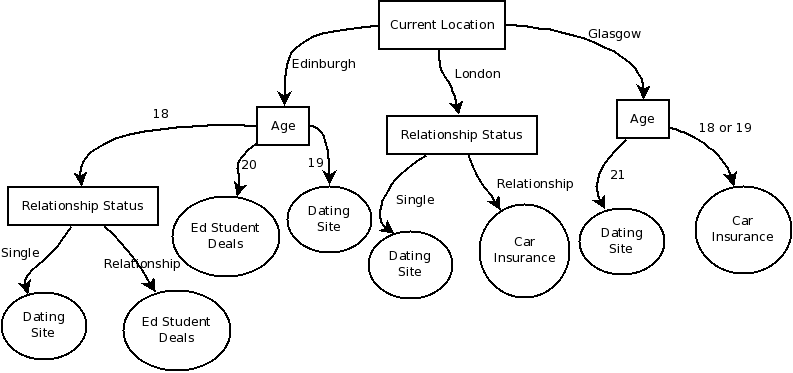
\includegraphics[scale=0.6]{Tree.png} 
     \end{figure}
   
     \newpage
   \section{An Unclassified Example}
     Below, we have the essential details of a person on Facebook. The year of their birth is assumed to be the same as
     mine (1990).
     
     \begin{figure}[H]
       \begin{center}
         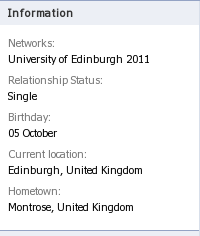
\includegraphics[scale=0.6]{Facebook.png}
       \end{center}
       \caption{A Facebook pages statistics}
     \end{figure}

     This person makes up a record that conforms to the tree built with my original training set.
     Their information in record form is below:

     \begin{table}[H] 
       \centering
       \caption{An Unclassified Record}
       \begin{tabular}{|c|c|c|c|c||c|}
         \hline
         \textbf{Record} & \textbf{RS} & \textbf{CL} &\textbf{Education} & \textbf{Age} & \textbf{Selected Advert} \\
          \hline
          15 & Single    &Edinburgh  & University & 20 & ? \\
          \hline
       \end{tabular}
     \end{table}
 
     Classifying them with the tree will follow this path (with the subscript showing the choice made at each decision point):

     \begin{equation}
       \mathrm{Current\; Location}_{Edinburgh} \rightarrow \mathrm{Age}_{20} \rightarrow \mathrm{Edinburgh\; Student\; Deals} 
     \end{equation}

     This shows that the tree correctly classifies the instance as a page that should be displaying the Edinburgh Student
     Deals advert.

  \section{Final Comments}
    This tree uses a continuous data field for classification. This may have been a mistake because I don't think that
    the techniques I used in creating the tree were really meant for handling fields with continuous values. For instance,
    if the example record had an age of 21, the tree wouldn't have been able to classify it. Another classification strategy
    should really have been used.

    As far as the rest of the coursework goes, I enjoyed it all immensely and even though I ran ID3 by hand to make the tree,     it wasn't as much effort as I thought it would be.                                             
    
\end{document}
